\documentclass[FIPLY_base.tex]{subfiles}

%\author{Daniel Bersenkowitsch}
\begin{document}
	\section{Pflichtenheft}
	
	\subsection{Motivation}
	Das Projekt wird im Rahmen einer Diplomarbeit durchgeführt.
	\subsection{Ausgangssituation und Zielsetzung}
	\subsubsection{Ausgangssituation}
	Fitnessapps gibt es wie Sand am Meer. Die Meisten davon sind nach demselben Prinzip aufgebaut: Es werden eine Reihe von Übungen vorgestellt und deren Ausführung beschrieben, meist nur in Textform. Der User kann sich anhand dieses Übungskatalogs sein Workout selbst zusammenstellen. Jedoch wissen vor allem Anfänger oft nicht, in welcher Intensität und in welcher Reihenfolge ein Training sinnvoll ist. 
	\subsubsection{Beschreibung des Geschäftsfeldes}
	Die Applikation kann von jedem benutzt werden, der körperlich aktiv sein will. Der Benutzer lädt sich die Applikation vom Google PlayStore herunter, gibt sein persönliches Profil und Trainingsziel an und erhält seinen angepassten Trainingsplan. Die App kann sowohl zu Hause als auch im Fitness-Studio verwendet werden. Nach jeder Trainingseinheit werden seine Fortschritte vermerkt und können eingesehen werden.
	
	\subsubsection{Zielbestimmung}
	Der User soll bei dem Verfolgen seiner Ziele (Muskelaufbau, Gesundheit, Abnehmen) durch die App unterstützt werden.
	
	\subsection{Funktionale Anforderungen}
	Die persönlichen Profildaten werden beim ersten Öffnen der Applikation erfasst. Der Benutzer kann jederzeit einen Trainingskatalog einsehen, in der alle Übungen grafisch nach Muskelgruppen sortiert sind. Jede Übung besitzt eine detaillierte Beschreibung, Anleitung und ein Video der Ausführung. Sobald man alle nötigen Informationen angegeben hat, ist es möglich einen Trainingsplan generieren zu lassen, welcher  als Excel-Tabelle abgespeichert und verschickt werden kann. Wenn man zu trainieren beginnen möchte, kann man eine Trainingssession starten. Dabei gibt es einen eingebauten Musikplayer, der die lokale Musikbibliothek wiedergibt. Die aktuelle Übung wird angezeigt und weiters steht ein Timer zur Verfügung, der vor allem beim Konditionstraining zum Einsatz kommt. Nach jedem Trainingsablauf soll der Benutzer ein Feedback geben, um seine Fortschritte zu vermerken. Die Fortschritte können jederzeit eingesehen und auf Social Networks geteilt werden. Zusätzlich werden einmal wöchentlich Userdaten (z.B.: Gewicht und Gesundheitszustand) abgefragt, um seine Entwicklung akkurat darstellen zu können.
	
	\subsubsection{Systemarchitektur}
	\begin{figure}[H]
		\begin{subfigure}[b]{0.3\textwidth}
			\centering
			%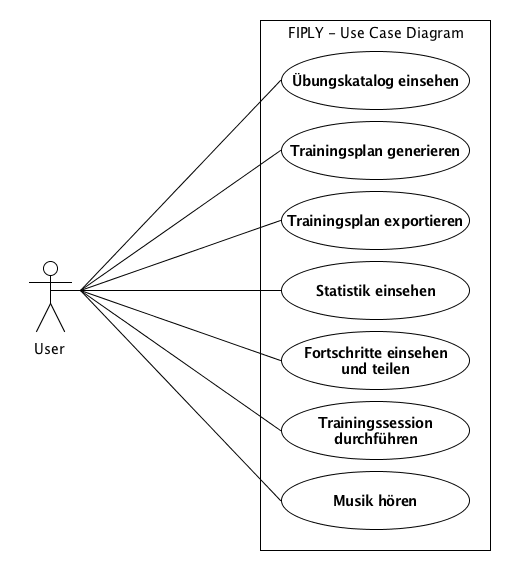
\includegraphics[scale=0.5]{img/UseCaseDiagram}
			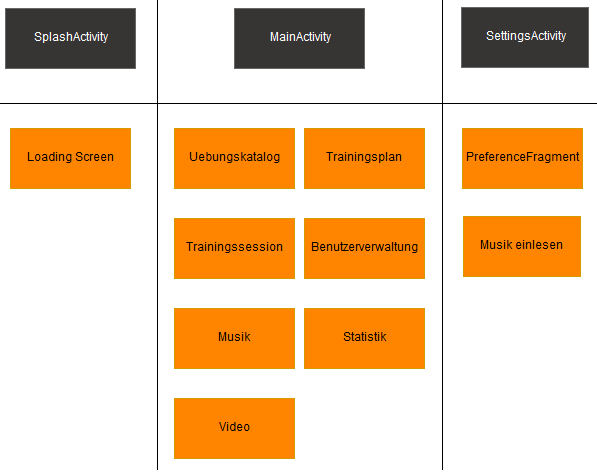
\includegraphics[scale=0.6]{img/Systemarchitektur}
		\end{subfigure}
		\caption{Das Use-Case Diagramm zu der Applikation}
	\end{figure}
	\newpage
	\subsubsection{Use Case Diagram (1 bis 6)}
	\begin{figure}[H]
		\begin{subfigure}[b]{0.3\textwidth}
			\centering
			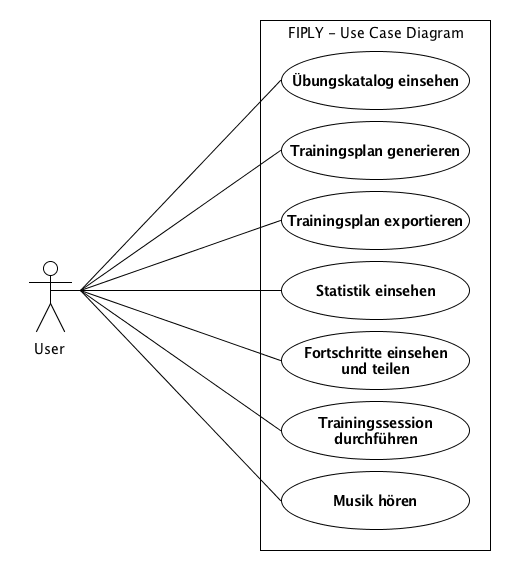
\includegraphics[scale=0.75]{img/UseCaseDiagram}
		\end{subfigure}
		\caption{Die Systemarchitektur zu der Applikation}
	\end{figure}
	\newpage
	\subsubsection{Use Case Details}
	UseCase 1: Übungskatalog einsehen
		\ \\
	\begin{center}
		\def\arraystretch{1.3}%
		\begin{tabular}{| p{3cm} | p{7cm} |}
			\hline
			UseCase 1: & Übungskatalog einsehen
			\\ \hline 
			Ziel des Use Cases: & Dem Benutzer soll eine Übersicht über alle Übungen geboten werden, falls er manuell einen Trainingsplan zusammenstellen oder sich über Übungen informieren will.
			\\ \hline
			Umgebende Systemgrenze: & Die Applikation selbst ist die Systemgrenze.
			\\ \hline
			Vorbedingung: & Keine.  
			\\ \hline
			Nachbedingung bei erfolgreicher Ausführung: & Keine.
			\\ \hline
			Beteiligte Nutzer: & Der Benutzer der App.
			\\ \hline
			Auslösendes Ereignis: & Durch das Betätigen des Knopfes „Übungen“.
			\\ \hline
		\end{tabular} \\
	\end{center}
		\ \\
	\begin{figure}[H]
		\begin{subfigure}[b]{0.3\textwidth}
			\centering
			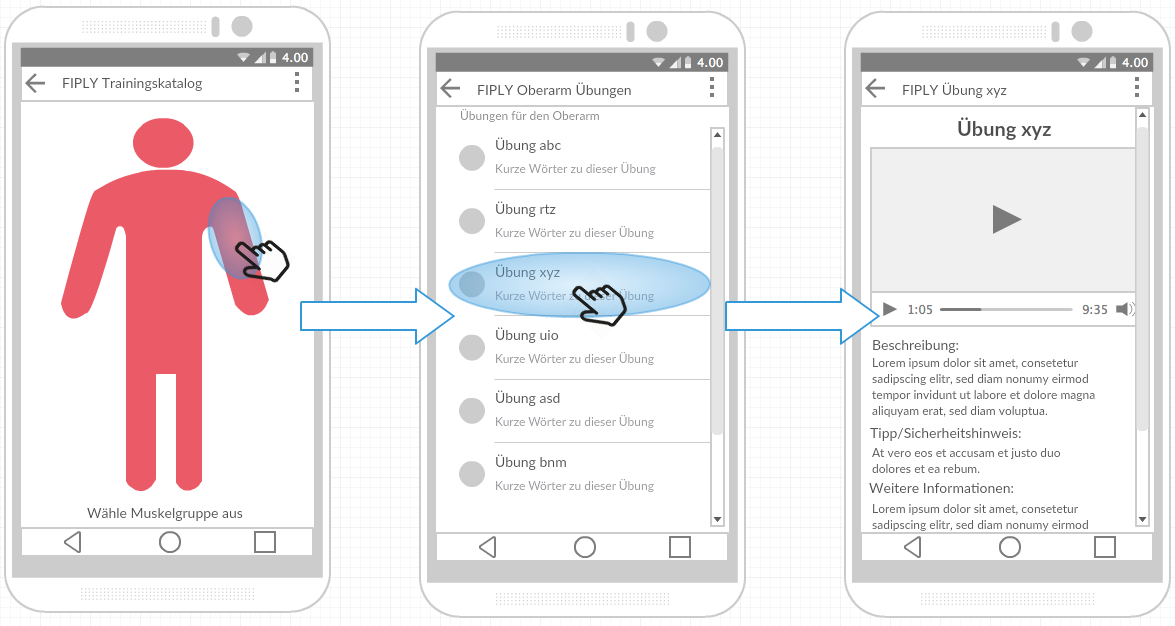
\includegraphics[scale=0.32]{img/Trainingskatalog}
		\end{subfigure}
		\caption{	GUI für den Aufruf/Ablauf des 1. Use Cases:}
	\end{figure}
		\ \\
	\begin{figure}[H]

		\begin{subfigure}[b]{0.3\textwidth}
			\centering
			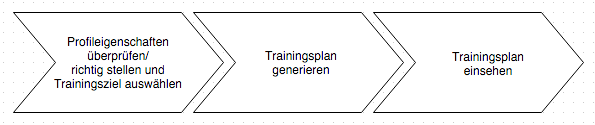
\includegraphics[scale=0.65]{img/TrainingsplanGenerierenLassen}
		\end{subfigure}
		\caption{Prozesskette des 1. Use Cases:}
	\end{figure}
		\ \\
	Szenario für den Standardablauf: (Erfolg)
		\ \\
	\begin{center}	
		\def\arraystretch{1.3}%
		\begin{tabular}{| p{4cm} |  p{4cm} |  p{4cm} |}
			\hline
			\textbf{Schritt} & \textbf{Nutzer} & \textbf{Beschreibung der Aktivität}
			\\ \hline 
			1: Trainingskatalog Übersicht wird geöffnet. & Der Benutzer der App. & Es wird grafisch eine Menschenfigur angezeigt und der Benutzer wird gebeten einen Körperteil auszuwählen um die spezifischen Übungen einzusehen.
			\\ \hline
			2: Anzeigen der Übungen. & Der Benutzer der App. & Es wird eine Liste von Übungen angezeigt, die der gewählten Muskelgruppe entsprechen. 
			\\ \hline
			3: Anzeigen einer ausgewählten Übung. & Der Benutzer der App. & Es wird ein kurzes Video zur korrekten Ausführung der Übung präsentiert, inklusive Beschreibung, Tipps bzw. Sicherheitshinweise und eventuellen weiteren Informationen.
			\\ \hline
		\end{tabular} \\
	\end{center}
	%\ \\
	%\begin{center}
	%	\line(1,0){380}
	%\end{center}
		%\ \\
		\newpage
	UseCase 2: Trainingsplan
		\ \\
	\begin{center}
		\def\arraystretch{1.3}%
		\begin{tabular}{| p{5cm} | p{5cm} |}
			\hline
		    UseCase 2: & Trainingsplan
			\\ \hline 
			Ziel des Use Cases: & Dem Benutzer soll ein individuell zusammengestellter Trainingsplan zur Verfügung gestellt werden. 
			\\ \hline
			Umgebende Systemgrenze: & Die Applikation selbst ist die Systemgrenze. 
			\\ \hline
			Vorbedingung: & Alle benötigten Profildaten (Größe, Gewicht, Geschlecht, Trainingsziel) müssen angegeben werden.  
			\\ \hline
			Nachbedingung bei erfolgreicher Ausführung: & Keine.  
			\\ \hline
			Beteiligte Nutzer: & Der Benutzer der App. 
			\\ \hline
			Auslösendes Ereignis: & Durch das betätigen des Knopfes „Trainingsplan“. 
			\\ \hline
		\end{tabular} \\
	\end{center}
		\ \\
	\begin{figure}[H]
		\begin{subfigure}[b]{0.3\textwidth}
			\centering
			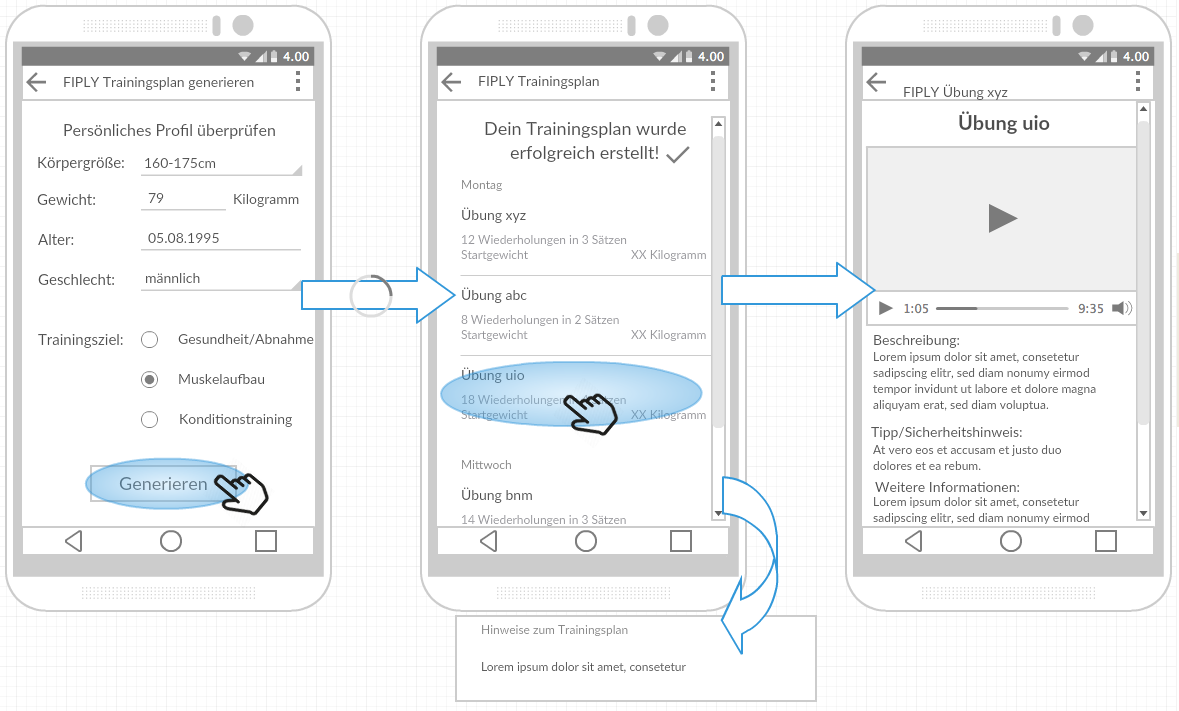
\includegraphics[scale=0.32]{img/Trainingsplangenerieren}
		\end{subfigure}
		\caption{GUI für den Aufruf/Ablauf des 2. Use Cases:}
	\end{figure}
		\ \\
	\begin{center}
		\def\arraystretch{1.3}%
		\begin{tabular}{| p{5cm} | p{5cm} |}
			\hline
			\textbf{Eingabefeld} & \textbf{Erlaubte Eingabewerte}
			\\ \hline 
			Körpergröße (slider) & 100 bis 200 (Zentimeter) 
			\\ \hline
			Gewicht (slider) & 40 bis 140 (Kilogramm)
			\\ \hline
			Alter (drop-down menu) & 16 bis 20,
					21 bis 30,
					31 bis 40,
					41 bis 50,
					51+
			\\ \hline
			Geschlecht (Drop-Down Menü) & männlich, weiblich, anderes
			\\ \hline
			Körperbau (Drop-Down Menü) & fit (trainiert), not fit (untrainiert)
			\\ \hline
		\end{tabular} \\
	\end{center}
		\ \\
	Szenario für den Standardablauf: (Erfolg)
	\begin{center}
		\def\arraystretch{1.3}%	
		\begin{tabular}{| p{4cm} | p{4cm} | p{4cm} |}
			\hline
			\textbf{Schritt} & \textbf{Nutzer} & 
			\textbf{Beschreibung der Aktivität} 
			\\ \hline 
			1: Daten des persönlichen Profils überprüfen. & Der Benutzer der App. & Die Daten werden vom Benutzer überprüft und wenn nötig angepasst. Nach der Bestimmung des Trainingsziels kann der Trainingsplan generiert werden.
			\\ \hline  
			2: Einsehen des generierten Trainingsplan. & Der Benutzer der App. & Der Trainingsplan wird nun angezeigt. 
			\\ \hline
			3: Anzeigen einer ausgewählten Übung. & Der Benutzer der App. & Es wird eine detaillierte Beschreibung, eine Anleitung und ein Video der Ausführung angezeigt.  \\ \hline
		\end{tabular} \\
	\end{center}
	\ \\
	Szenarien für alternative Abläufe: (Misserfolg oder Umwege zum Erfolg)
		\ \\
	\begin{center}
		\def\arraystretch{1.3}%	
		\begin{tabular}{| p{2cm} | p{4cm} | p{4cm} |}
			\hline
			\textbf{Schritt} & \textbf{Bedingung, unter der Alternative eintritt} & \textbf{Beschreibung der Aktivität} 
			\\ \hline 
			1 & Falsche Eingabe bei den Eingabefeldern & Die App fordert den Nutzer auf seine fehlerhaften Daten anzupassen.\\ \hline
		\end{tabular} \\
	\end{center}
	%	\ \\
	%\begin{center}
	%	\line(1,0){380}
	%\end{center}
		%\ \\
	UseCase 3: Trainingsplan exportieren lassen
	\ \\
	\begin{center}
		\def\arraystretch{1.3}%
		\begin{tabular}{| p{5cm} | p{5cm} |}
			\hline
			UseCase 3: & Trainingsplan exportieren lassen \\ \hline 
			Ziel des Use Cases: & Es soll gewährleistet werden, dass der Benutzer auch ohne Smartphone trainieren gehen kann. \\ \hline
			Umgebende Systemgrenze: & Die Applikation selbst ist die Systemgrenze. \\ \hline
			Vorbedingung: & Ein Trainingsplan muss bereits erstellt worden sein (Use Case 2).  \\ \hline
			Nachbedingung bei erfolgreicher Ausführung: & Keine. \\ \hline
			Beteiligte Nutzer: & Der Benutzer der App. \\ \hline
			Auslösendes Ereignis: & Durch das Betätigen des Knopfes „Exportieren“. \\ \hline
		\end{tabular} \\
	\end{center}
		\ \\
	\begin{figure}[H]
		\begin{subfigure}[b]{0.3\textwidth}
			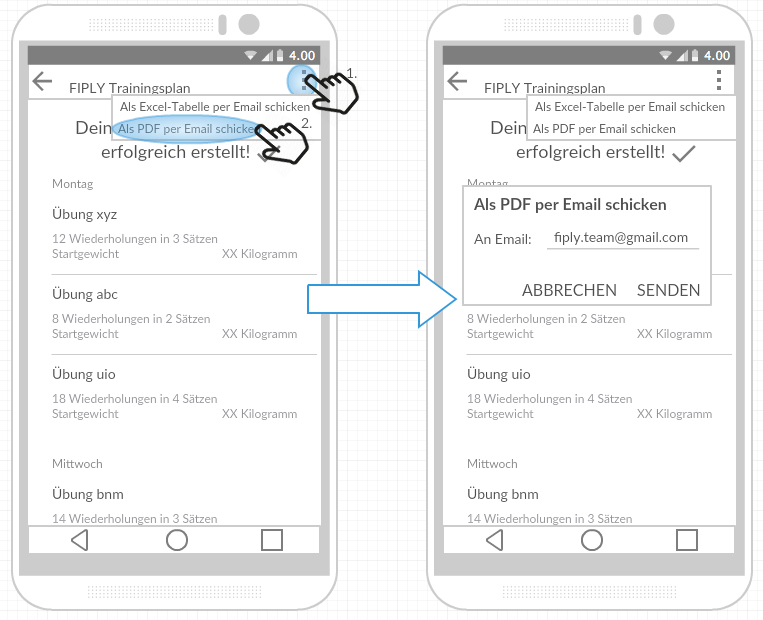
\includegraphics[scale=0.32]{img/Trainingsplanexportieren}
		\end{subfigure}
		\caption{GUI für den Aufruf/Ablauf des 3. Use Cases:}
	\end{figure}
		\ \\
	\begin{center}
		\def\arraystretch{1.3}%
		\begin{tabular}{| p{5cm} | p{5cm} |}
			\hline
			\textbf{Eingabefeld:} & \textbf{Erlaubte Eingabewerte} \\ \hline 
			Email & Korrekte Emailadresse \\ \hline
		\end{tabular} \\
	\end{center}
	\ \\
	Szenario für den Standardablauf: (Erfolg)
	\begin{center}	
		\def\arraystretch{1.3}%
		\begin{tabular}{| p{4cm} | p{4cm} | p{4cm} |}
			\hline
			\textbf{Schritt} & \textbf{Nutzer} & \textbf{Beschreibung der Aktivität}  \\ \hline 
			1: Der Benutzer will den Trainingsplan exportieren. & Der Benutzer der App. & Der Trainingsplan wird als Excel-Tabelle exportiert.\\ \hline
			2: Email angeben. & Der Benutzer der App. & Die Emailadresse an die die Datei gesendet werden soll wird angegeben.  \\ \hline
		\end{tabular} \\
	\end{center}
	\ \\
	Szenarien für alternative Abläufe (Misserfolg oder Umwege zum Erfolg)
	\begin{center}
		\def\arraystretch{1.3}%	
		\begin{tabular}{| p{4cm} | p{4cm} | p{4cm} |}
			\hline
			\textbf{Schritt} & \textbf{Bedingung, unter der Alternative eintritt} & \textbf{Beschreibung der Aktivität}  \\ \hline 
			2: Email angeben & Irrtum des Benutzers. & In das Email Textfeld wird eine nicht formatkorrekte Email angegeben.\\ \hline
		\end{tabular} \\
	\end{center}
	\ \\
	\begin{figure}[h]
		\begin{subfigure}[b]{0.3\textwidth}
			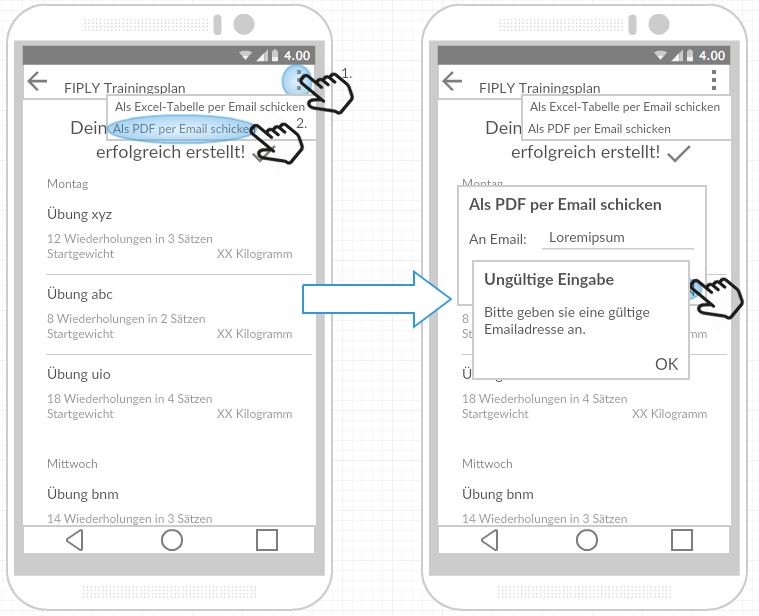
\includegraphics[scale=0.32]{img/TrainingsplanexportierenungueltigeEingabe}
		\end{subfigure}
		\caption{GUIs für  den alternative Abläufe des Use Cases:}
	\end{figure}
	\ \\
	\begin{center}
		\def\arraystretch{1.3}%	
		\begin{tabular}{| p{5cm} | p{5cm} |}
			\hline
			\textbf{Eingabefeld:} & \textbf{Erlaubte Eingabewerte} \\ \hline 
			Email (Textfeld) & Gültige ist eine formatkorrekte Emailadresse. Alles andere wird als nicht valide erkannt. \\ \hline
		\end{tabular} \\
	\end{center}
	%\ \\
	%\begin{center}
	%	\line(1,0){380}
	%\end{center}
	%\ \\
	\newpage
	UseCase 4: Trainingssession durchführen und Musik hören.
	\ \\
	\begin{center}
		\def\arraystretch{1.3}%	
		\begin{tabular}{| p{5cm} | p{5cm} |}
			\hline
			UseCase 4: & Trainingssession durchführen und Musik hören. \\ \hline 
			Ziel des Use Cases: & Der Benutzer bleibt beim Trainieren konzentriert, kann seine Fortschritte festhalten und wird zusätzlich durch die Musik motiviert. \\ \hline
			Umgebende Systemgrenze: & Die Applikation selbst ist die Systemgrenze. \\ \hline
			Vorbedingung: & Ein Trainingsplan muss aufbereitet worden sein (Use Case 3).  \\ \hline
			Nachbedingung bei erfolgreicher Ausführung: & Keine.  \\ \hline
			Beteiligte Nutzer: & Der Benutzer der App. \\ \hline
			Auslösendes Ereignis: & Durch das Betätigen des Knopfes „Training“. \\ \hline
		\end{tabular} \\
	\end{center}
	GUI für den Aufruf/Ablauf des Use Cases:
	\begin{figure}[H]
		\begin{subfigure}[b]{0.3\textwidth}
			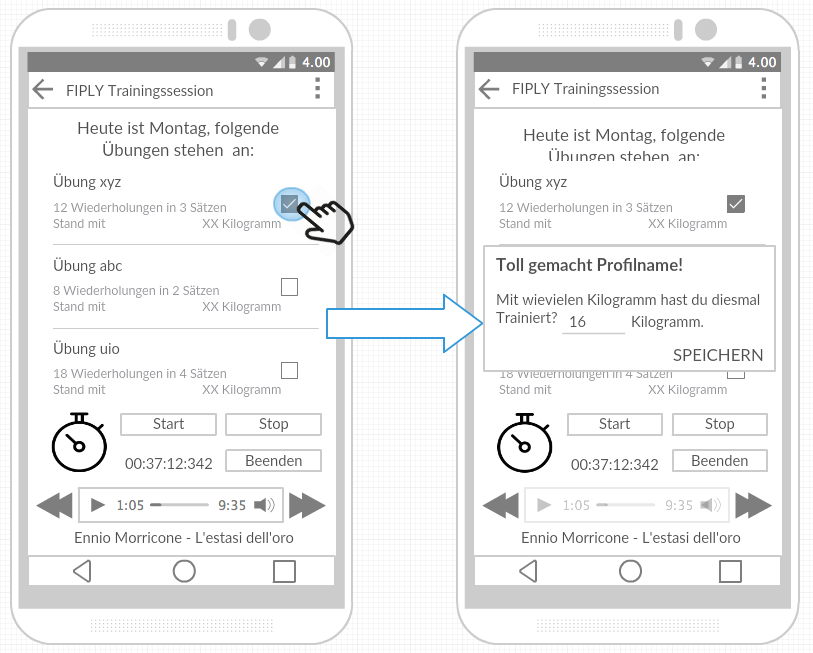
\includegraphics[scale=0.32]{img/TrainingssessionUebungabgeschlossen}
		\end{subfigure}
		\caption{GUI für den Aufruf/Ablauf des 4. Use Cases:}
	\end{figure}
	\begin{center}
		\def\arraystretch{1.3}%	
		\begin{tabular}{| p{5cm} | p{5cm} |}
			\hline
			\textbf{Eingabefeld:} & \textbf{Erlaubte Eingabewerte} \\ \hline 
			Kilogramm (Textfeld) & 40 bis 140 \\ \hline
		\end{tabular} \\
	\end{center}	
	\begin{figure}[H]
		\begin{subfigure}[b]{0.3\textwidth}
			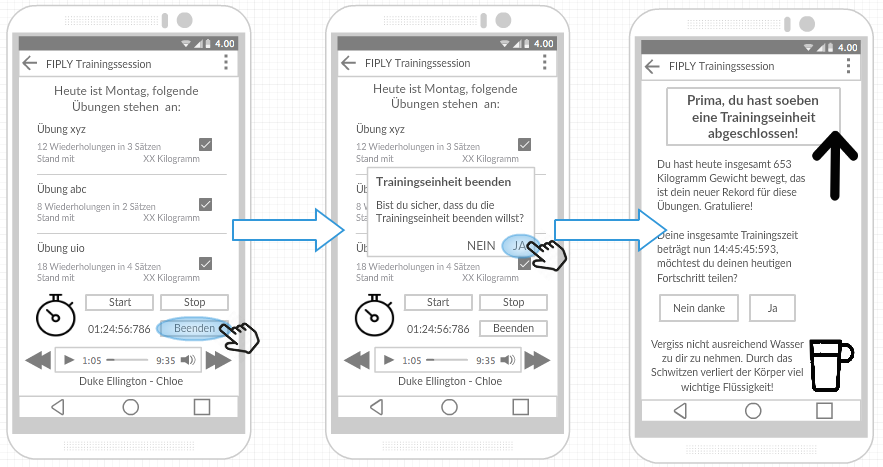
\includegraphics[scale=0.4]{img/Trainingssessionabgeschlossen}
		\end{subfigure}
		\caption{GUI für den Aufruf/Ablauf des 4. Use Cases:}
	\end{figure}
	Szenario für den Standardablauf: (Erfolg)
	\begin{center}	
		\def\arraystretch{1.3}%	
		\begin{tabular}{| p{4cm} | p{3cm} | p{5cm} |}
			\hline
			\textbf{Schritt} & \textbf{Nutzer} & \textbf{Beschreibung der Aktivität}  \\ \hline 
			1: Starten des Musikplayers. & Der Benutzer der App. & Die Applikation spielt ein Lied aus der lokalen Musikbibliothek ab.\\ \hline
			2: Ausführen der Übungen. & Der Benutzer der App. & Der Benutzer führt nun die anstehenden Übungen aus. \\ \hline
			3: Eine Übung abschließen. & Der Benutzer der App. & Sobald eine Übung abgeschlossen ist, kann er per Knopfdruck zur nächsten Übung springen.  \\ \hline
			4: Trainingseinheit abschließen. & Der Benutzer der App. & Wenn alle Übungen abgeschlossen sind und der „Trainingsession beenden“-Knopf gedrückt wurde, wird sein Trainingserfolg wiedergegeben.  \\ \hline
		\end{tabular} \\
	\end{center}
	\ \\
	Szenarien für alternative Abläufe: (Misserfolg oder Umwege zum Erfolg)
	\ \\
	\begin{center}	
		\def\arraystretch{1.3}%	
		\begin{tabular}{| p{4cm} | p{4cm} | p{4cm} |}
			\hline
			\textbf{Schritt} & \textbf{Bedingung, unter der Alternative eintritt} & \textbf{Beschreibung der Aktivität}  \\ \hline 
			Es wird eine Übung angeklickt. & Der Benutzer kennt die Übung nicht oder will sie einsehen. & Die Übung wird während einer Trainingseinheit angeklickt und die Details dazu werden geöffnet.\\ \hline
		\end{tabular} \\
	\end{center}
	\ \\
	GUIs für  den alternative Abläufe des Use Cases:
	\ \\
	\begin{figure}[H]
		\begin{subfigure}[b]{0.3\textwidth}
			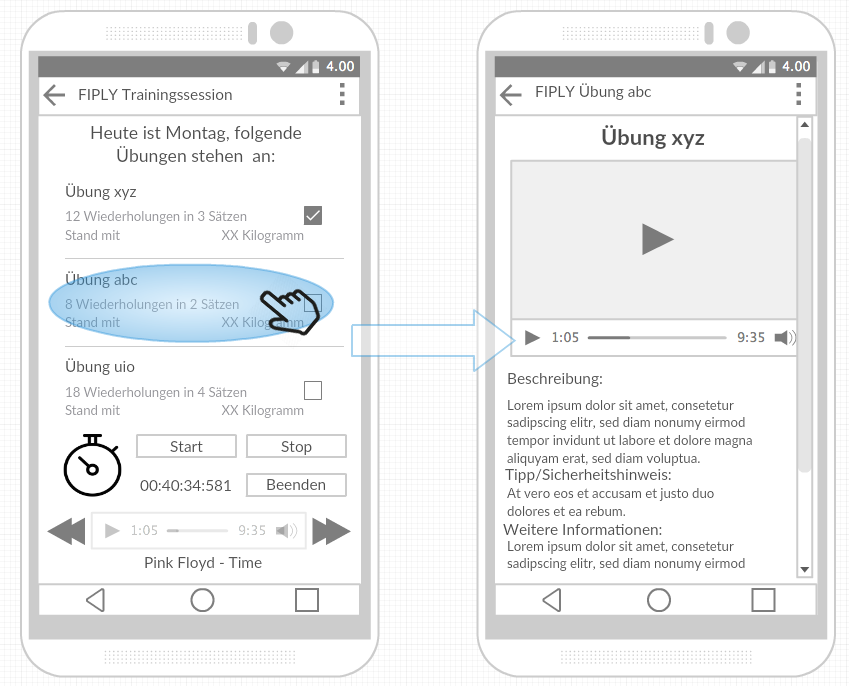
\includegraphics[scale=0.32]{img/Trainingssessionalternativ}
		\end{subfigure}
		\caption{GUI für den alternativen Aufruf/Ablauf des 4. Use Cases:}
	\end{figure}
	\ \\
	Das Startgewicht ist das Gewicht mit dem der Benutzer am Anfang üben soll. Sobald  er mit schwereren Gewichten zu trainieren beginnt, kann er die Veränderung eintragen. Dies wird dann in der Trainingsentwicklung gespeichert. 
	
	%\begin{center}
	%	\line(1,0){380}
	%\end{center}
	%\ \\
	\newpage
	UseCase 5: Fortschritte/Statistik anzeigen lassen.
	\ \\
	\begin{center}
		\def\arraystretch{1.3}%	
		\begin{tabular}{| p{5cm} | p{5cm} |}
			\hline
			UseCase 5: & Fortschritte/Statistik anzeigen lassen. \\ \hline 
			Ziel des Use Cases: & Der Benutzer soll durch die Visualisierung seiner Fortschritte motiviert werden. \\ \hline
			Umgebende Systemgrenze: & Die Applikation selbst ist die Systemgrenze. \\ \hline
			Vorbedingung: & Keine.  \\ \hline
			Nachbedingung bei erfolgreicher Ausführung: & Keine.  \\ \hline
			Beteiligte Nutzer: & Der Benutzer der App. \\ \hline
			Auslösendes Ereignis: & Durch das Betätigen des Knopfes „Statistik“. \\ \hline
		\end{tabular} \\
	\end{center}
	\ \\ 
	GUI für den Aufruf/Ablauf des Use Cases:
	\begin{figure}[H]
		\begin{subfigure}[b]{0.3\textwidth}
			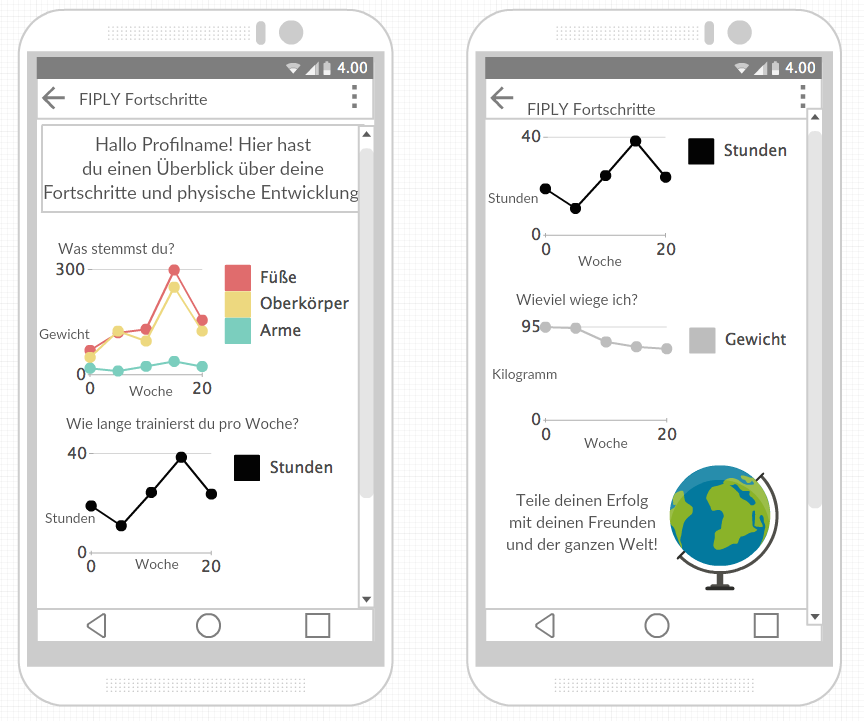
\includegraphics[scale=0.32]{img/Fortschrittsanzeige}
		\end{subfigure}
		\caption{GUI für den alternativen Aufruf/Ablauf des 5. Use Cases:}
	\end{figure}
	\newpage
	Szenario für den Standardablauf: (Erfolg)
	\ \\
	\begin{center}	
		\def\arraystretch{1.3}%	
		\begin{tabular}{| p{4cm} | p{4cm} | p{4cm} |}
			\hline
			\textbf{Schritt} & \textbf{Nutzer} & \textbf{Beschreibung der Aktivität}  \\ \hline 
			1: Einsehen der Fortschritte. & Der Benutzer der App. & Anzeige der Momentanaufnahmen aus den Trainingssessions.\\ \hline
		\end{tabular} \\
	\end{center}
	
	UseCase 6: Fortschritte auf Facebook teilen.
	\begin{center}
		\def\arraystretch{1.3}%	
		\begin{tabular}{| p{5cm} | p{5cm} |}
			\hline
			UseCase 6: & Fortschritte/Statistik anzeigen lassen. \\ \hline 
			Ziel des Use Cases: & Dadurch soll eine Community aufgebaut werden und andere dazu motiviert werden die Applikation auch zu benutzen.  \\ \hline
			Umgebende Systemgrenze: & Die Applikation selbst ist die Systemgrenze. \\ \hline
			Vorbedingung: & Ein oder mehrere Trainingssessions müssen durchgeführt worden sein.  \\ \hline
			Nachbedingung bei erfolgreicher Ausführung: & Keine.  \\ \hline
			Beteiligte Nutzer: & Der Benutzer der App. \\ \hline
			Auslösendes Ereignis: & Durch das Betätigen des Knopfes „Erfolg teilen“. \\ \hline
		\end{tabular} \\
	\end{center}
	GUIs für den Aufruf/Ablauf des Use Cases:
	\begin{figure}[H]
		\begin{subfigure}[b]{0.3\textwidth}
			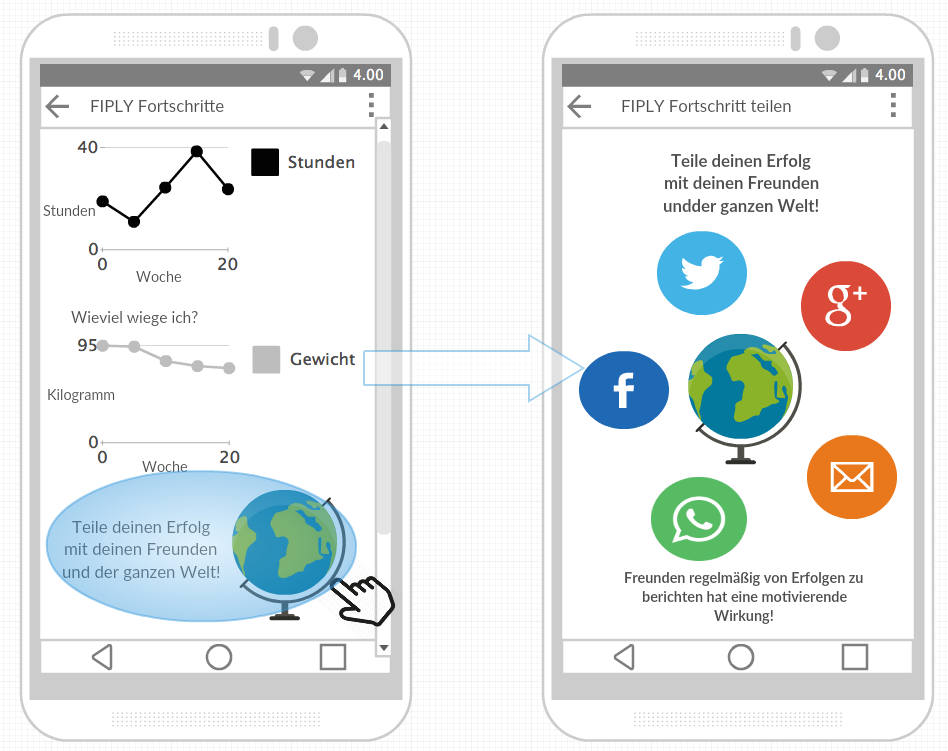
\includegraphics[scale=0.32]{img/Fortschrittteilen1}
		\end{subfigure}
		\caption{GUI für den Aufruf/Ablauf des 6. Use Cases:}
	\end{figure}
	\begin{figure}[H]
		\begin{subfigure}[b]{0.3\textwidth}
			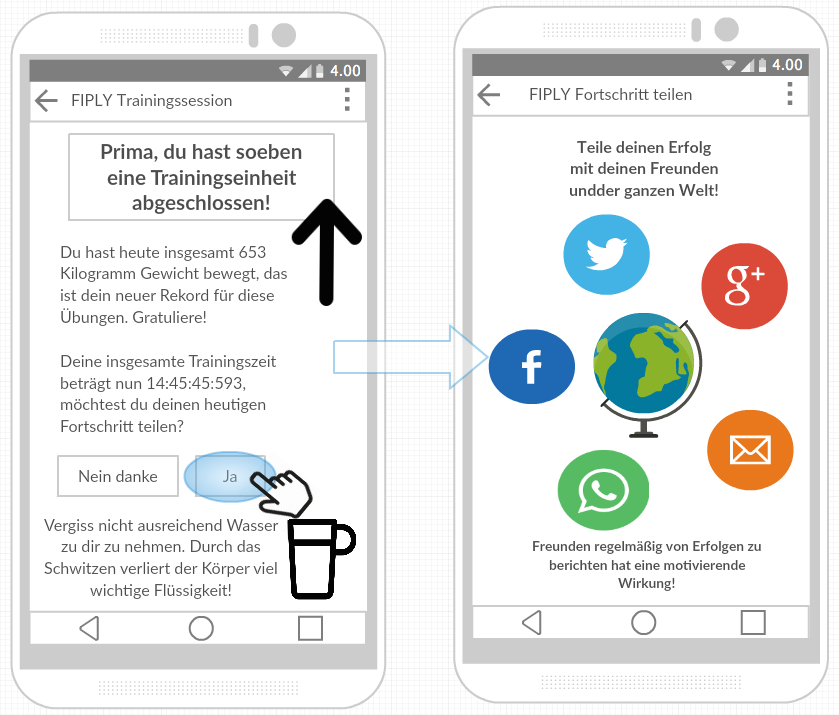
\includegraphics[scale=0.32]{img/Fortschrittteilen2}
		\end{subfigure}
		\caption{GUI für den Aufruf/Ablauf des 6. Use Cases:}
	\end{figure}
	
	\newpage
	\subsection{Nicht-funktionale Anforderungen}
	\begin{center}
		\def\arraystretch{1.3}%	
		\begin{tabular}{| p{5cm} | p{5cm} |}
			\hline
			Name: & Intuitive Oberfläche \\ \hline 
			Typ: & USE \\ \hline
			Beschreibung: & Die Applikation soll leicht bedienbar sein. Übersichtliches Design. \\ \hline
			Zugeordnete Use Cases & 1,2,3,4,5 und 6.  \\ \hline
		\end{tabular} \\
	\end{center}
	\begin{center}
		\def\arraystretch{1.3}%	
		\begin{tabular}{| p{5cm} | p{5cm} |}
			\hline
			Name: & Einfach verständlich für Fitnesslaien \\ \hline 
			Typ: & USE \\ \hline
			Beschreibung: & Auch Fitnesslaien sollen sich in der App zurechtfinden und nicht mit Fachbegriffen überfordert werden. \\ \hline
			Zugeordnete Use Cases & 1,2,4 und 6.  \\ \hline
		\end{tabular} \\
	\end{center}
	\begin{center}
		\def\arraystretch{1.3}%	
		\begin{tabular}{| p{5cm} | p{5cm} |}
			\hline
			Name: & Community einrichten \\ \hline 
			Typ: & USE \\ \hline
			Beschreibung: & Es soll eine Community auf Facebook aufgebaut werden, um die Nutzer motiviert zu halten. \\ \hline
			Zugeordnete Use Cases & 1,2,4 und 6.  \\ \hline
		\end{tabular} \\
	\end{center}
	\begin{center}
		\def\arraystretch{1.3}%	
		\begin{tabular}{| p{5cm} | p{5cm}  |}
			\hline
			Name: & Offlineverwendung \\ \hline 
			Typ: & USE \\ \hline
			Beschreibung: & Die Applikation soll auch ohne aktiver   Internetverbindung benutzbar sein. \\ \hline
			Zugeordnete Use Cases & 1,2,4 und 6  \\ \hline
		\end{tabular} \\
	\end{center}
	\ \\
	\subsection{Mengengerüst}
	Übungskatalog 50-100 Datensätze einmalig in die Übungskatalogtabelle (kaum neue Sätze).
	Trainingssession 100-200 Datensätze pro Jahr in die Trainingssession-Tabelle.
	Usersnapshot: 50-55 Datensätze pro Jahr in die Usersnapshot-Tabelle.
	50-100 Videos werden von Youtube eingebunden.
	Zusätzlich werden 50-200 komprimierte Fotos abgespeichert werden.
	
	\subsection{Risikovermeidung}
	Sollte Nutzer bei Verwendung der Apps psychische oder physische Schäden davontragen trägt er selbst die Verantwortung.
	
	\subsection{Abnahmekriterien}
	Die App ist im Google Playstore verfügbar.
	Man kann über eine intuitive Oberfläche ein Profil erstellen und sich einen Trainingsplan generieren lassen. Zusätzlich kann eine Trainingssession durchgeführt werden und Informationen über seine Entwicklung stehen zur Verfügung.
	Erfolge können über Facebook geteilt werden.
	
\end{document}